\section{Analyse der Tranceiver-Platinen}
Zu Verfügung steht eine Tranceiver-Platine. Ein Tranceiver ist eine Platine, die sowohl als Sender (Transmitter) als auch als Empfänger (Receiver) fungieren kann. Dafür ist diese Platine mit einem Transceiver-Chip ausgestattet, der Funktion teilweise abgeschaltet werden kann, sodass die Platine zu einem reinen Transmitter oder zu einem reinen Receiver wird.  
Hierfür stehen zwei Jumper zur Verfügung, die auf der Tranceiver-Platine platziert sind. Diese Jumper können gesteckt oder abgezogen werden, um die Funktionalität der Platine zu ändern. Hierbei ist der Platinenbeschriftung zu entnehmen, dass der TX (Transmitter) nur dann funktioniert, wenn man sowohl J1 und J2 ausgesteckt hat (eine Eingangsspannung liegt dann an dem Transceiver-Chip auf beiden Teilmodulen an). Jedoch ist das tatsächlich nicht der Fall,
wie es sich bei der Versuchsdurchführung herausstellt und lässt folgern, dass diese Beschriftung falsch ist.

Die Jumpers sind auf der Abbildung \ref{fig:Tranceiver-Platine} zu sehen.
\begin{figure}[H]
    \centering
    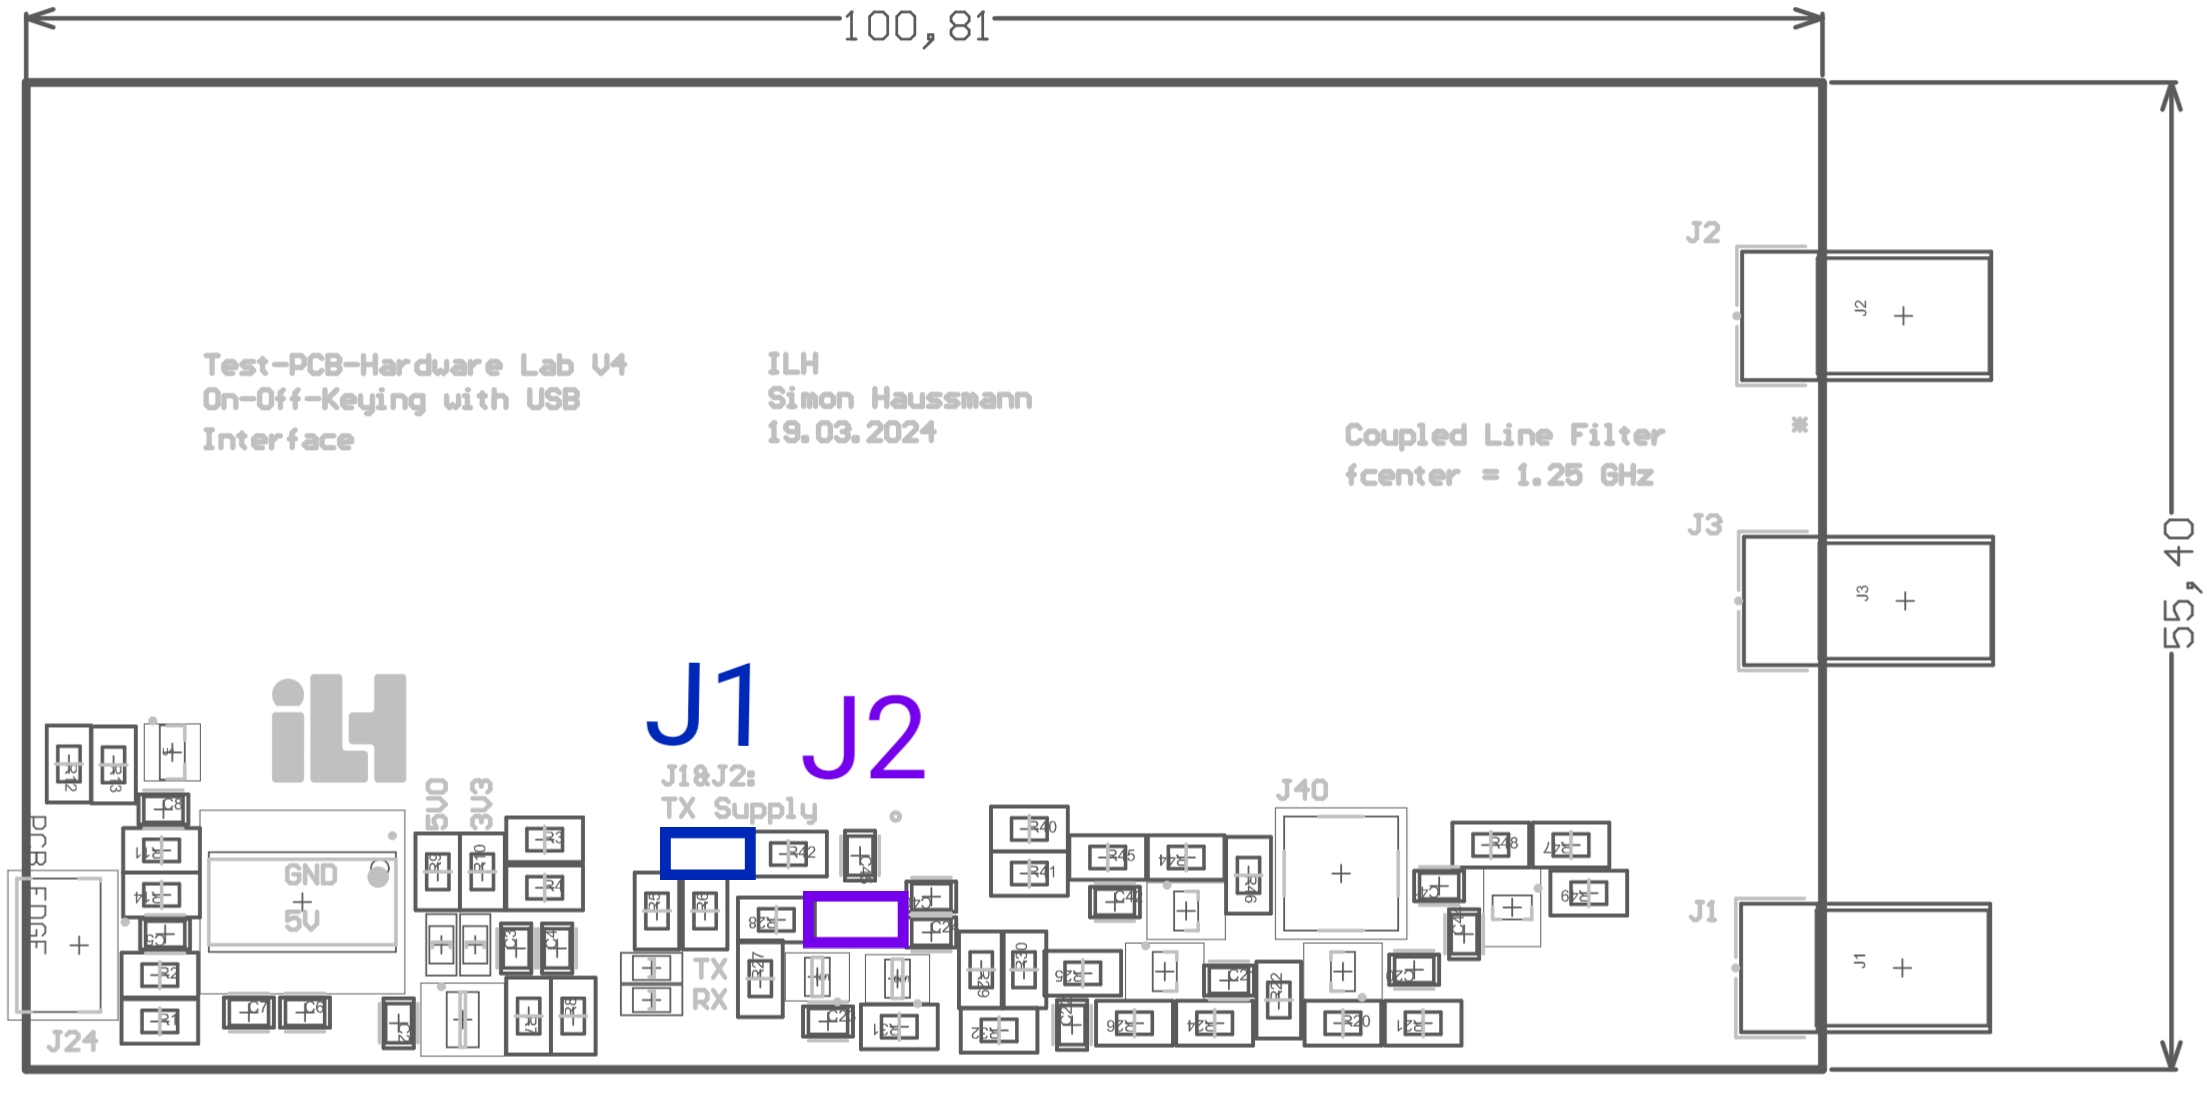
\includegraphics[width=0.8\textwidth]{Pictures/Jumper.jpg}
    \caption{Tranceiver-Platine mit Jumpern J1 und J2. Quelle: vgl. Litertaturverzeichnis \cite{SchaltplanPCBV4}: Schaltpläne der Platine V4}
    \label{fig:Tranceiver-Platine}
\end{figure}
\subsection{Funktion der Jumper}
\begin{figure}[H]
    \centering
    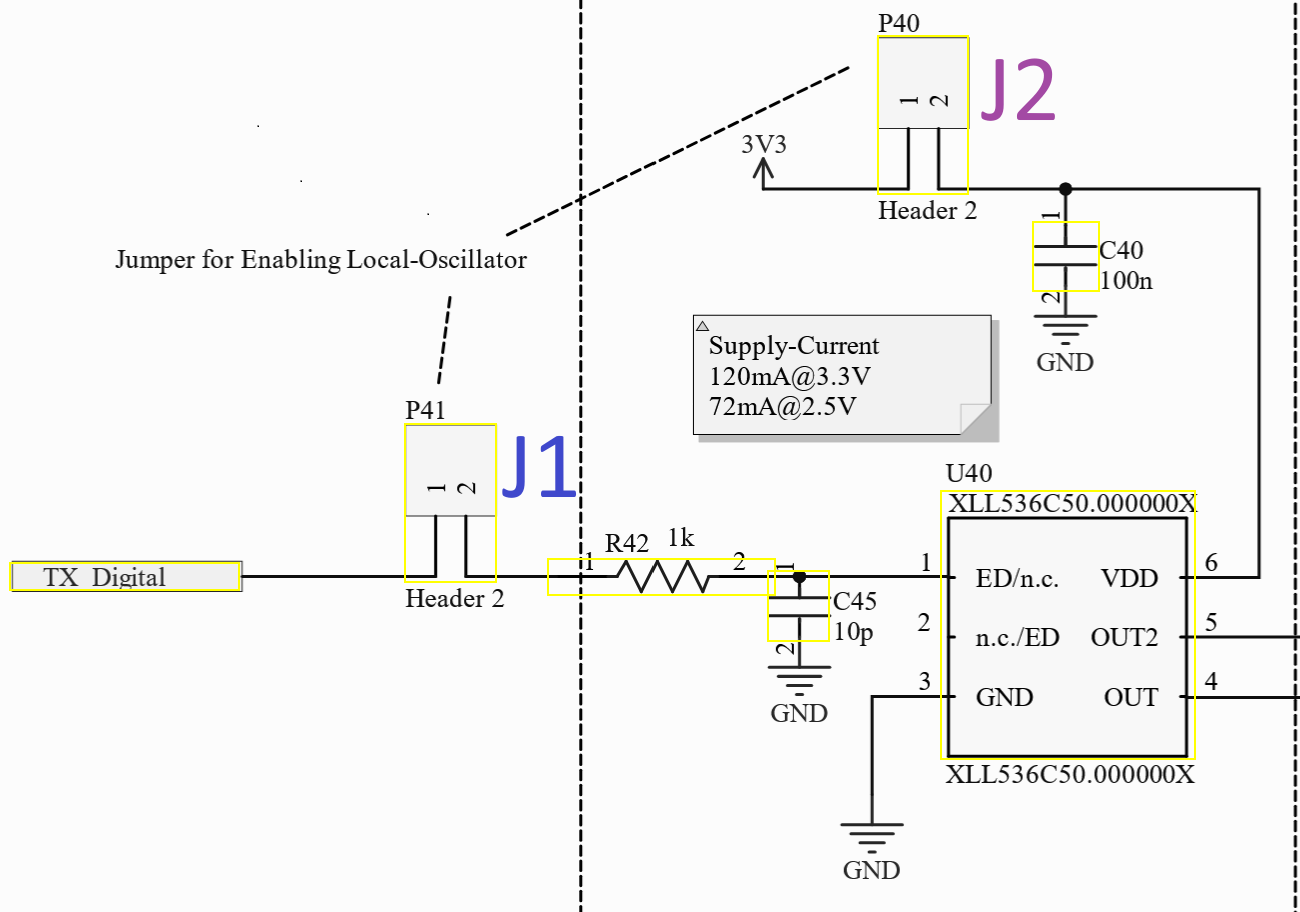
\includegraphics[width=0.8\textwidth]{Pictures/JumperSchaltung.png}
    \caption{Jumper auf der Tranceiver-Platine}
    \label{fig:Jumper}
\end{figure}
\subsection{J1}
Der Jumper J1 ist wie im Schaltplan zu sehen, der Schalter der den Oszilator enabled und disabled.
\subsection{J2}
Der Jumper J2 ist wie im Schaltplan zu sehen, der Schalter für die Versorgungsspannung des Oszilators.

Es ist auch wichtig zu beachten, dass ohne den Receiver der Transmitter nicht funktionieren kann. Das bedeutet, dass der Jumper J2 immer abgezogen sein muss, damit der Transmitter funktioniert. Dies ist auf die eingeschaften des zur Verfügung stehenden Transceiver-Chips zurückzuführen.

\subsection{Serielles Protokoll UART}
Universal Asynchronous Receiver/Transmitter (UART) stellt ein serielles Protokoll dar, also einen Regelsatz für den Austausch von Daten zwischen zwei Geräten. Das Protokoll ist asynchron, was bedeutet, dass es kein gemeinsamer Taktsignal zwischen dem Sender und dem Empfänger gibt. Stattdessen müssen beide Seite auf dieselbe Bit- und Baudrate eingestellt
Zudem müssen die beiden Seiten dieselbe Rahmenstruktur und dieselben Parameter nutzen. Das UART-Protokoll ist simpel und ermöglicht die Signalübertragung in beide Richtungen über lediglich zwei Drähte zwischen Sender und Empfänger. Das Signal wird in einem vom Protokoll bestimmten Format gesendet.\footnote{Vgl. Rohde \& Schwarz: UART verstehen. Online: \url{https://www.rohde-schwarz.com/de/produkte/messtechnik/essentials-test-equipment/digital-oscilloscopes/uart-verstehen_254524.html} (abgerufen am 07.07.2025).} 

Die Kommunikation über UART kann in verschiedenen Formaten, nämlich im:
\begin{itemize}
    \item Simplex-Betrieb
    \item Halbduplex-Betrieb
    \item Voll-Duplex-Betrieb
\end{itemize}
erfolgen.

Das Rahmenformat von UART sieht folgendermaßen aus:
\begin{figure}[H]
    \centering
    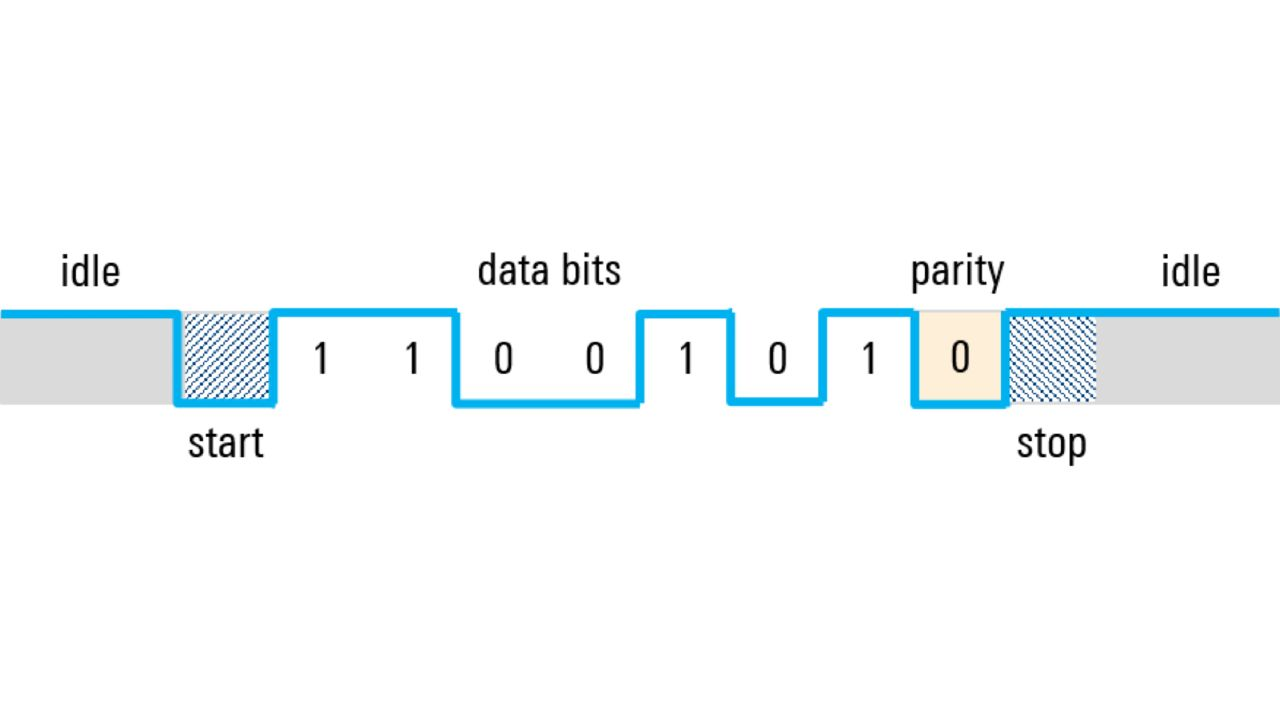
\includegraphics[width=0.8\textwidth]{Pictures/UART-Frame.jpg}
    \caption{Rahmenformat von UART. Quelle: \url{https://cdn.rohde-schwarz.com/image/products/test-and-measurement/essentials-test-equipment/essentials-digital-oscilloscopes/understanding-uart-02-infographic-rohde-schwarz_200_112521_1024_576_7.jpg}}
    \label{fig:UART-Frame}
\end{figure}

Die Übertragung erfolgt in Form von Bytes, die aus 8 Datenbits bestehen. UART-Rahmen enthalten Start- und Stoppbits und Datenbits, die die tatsächliche Information tragen. Wie bei den meisten digitalen Systemen ist es vom UART-Protokoll festgelegt, dass der HIGH-Pegel einer logischen "1" und der LOW-Pegel einer logischen "0" entspricht. Eine spezifische Spannungsschwelle ist aus Flexibilitätsgründen durch UART nicht festgelegt, weswegen der HIGH-Pegel als "Mark" und der LOW-Pegel als "Space" beschrieben wird. Doch es ist zu beachten, dass das System beim UART-Protokoll im Ruhezustand (engl. idle) bei einem HIGH-Pegel liegt. Dies hat den Sinn, dass man bei einer beschädigten Leitung durch einen konstanten LOW-Pegel im Ruhezustand eine defekte Leitung/Verbindung bzw. einen defekten Sender erkennen kann.\footnote{Vgl. Rohde \& Schwarz: UART verstehen. Online: \url{https://www.rohde-schwarz.com/de/produkte/messtechnik/essentials-test-equipment/digital-oscilloscopes/uart-verstehen_254524.html} (abgerufen am 07.07.2025).}

Der Startbit signalisiert den Beginn der Datenübertragung. Hierbei übergeht der Sender aus dem Ruhezustand (HIGH-Pegel) in den LOW-Pegel, um dem Empfänger zu signalisieren, dass die Datenübertragung beginnt. 
Unmittelbar danach folgen die Datenbits, die das Nutzsignal übertragen. Die Datenbits werden nacheinander gesendet, wobei eine Übertragung von 5 bis 9 Bits pro Byte erlaubt ist, jedoch eine Übertragung von 7 oder 8 Bits pro Byte am häufigsten verwendet wird. Die Reihenfolge der Datenbits wird dabei vom Sender invertiert und mit dem Least Significant Bit (LSB) zuerst gesendet. Das Most Significant Bit (MSB) wird zuletzt gesendet.
Nach einer erfolgreichen Übertragung der Nutzdaten übergeht der Sender zurück in den Ruhezustand (HIGH-Pegel), um dem Empfänger zu signalisieren, dass die Übertragung abgeschlossen ist.
In einigen Fällen kann es auch vorkommen, dass ein zweites (optionales) Stoppbit konfiguriert wird, um dem Empfänger Zeit für den nächsten Übertragungsrahmen zu gewähren. Dies wird jedoch in der Praxis selten umgesetzt.\footnote{Vgl. Rohde \& Schwarz: UART verstehen. Online: \url{https://www.rohde-schwarz.com/de/produkte/messtechnik/essentials-test-equipment/digital-oscilloscopes/uart-verstehen_254524.html} (abgerufen am 07.07.2025).}

Zuletzt sollte man noch erwähnen, dass manchmal ein Paritätsbit zur Verwendung kommt. Dieser trägt zur Fehlererkennung bei, indem es die Anzahl der gesetzten Bits (1-Bits) in einem Byte überprüft. Es gibt zwei Arten von Paritätsbits: 
\begin{itemize}
    \item Gerade Parität: Hier wird das Paritätsbit so gesetzt, dass die Gesamtanzahl der 1-Bits im Byte gerade ist.
    \item Ungerade Parität: Hier wird das Paritätsbit so gesetzt, dass die Gesamtanzahl der 1-Bits im Byte ungerade ist.
\end{itemize}

Das Paritätsbit kann jedoch nur ein einziges gekipptes (also falsch übertragenes) Bit erkennen, aber nicht korrigieren. Es kann auch nicht erkennen, ob zwei oder mehr Bits gekippt wurden. Daher ist es in der Praxis nicht sehr verbreitet und wird oft weggelassen.\footnote{Vgl. ebenda}

Bei unserer tatsächlichen Schaltung liegt auch ein Standard-UART-Protokoll vor, das eine Baudrate von 115200 Baud und eine Datenübertragung von 8 Datenbits, 1 Stoppbit und ohne Paritätsbit verwendet.

\subsubsection{Betriebsarten von UART}
Es gibt insgesamt drei Arten vom Betrieb des UART-Protokolls:
\begin{enumerate}
    \item \textbf{Simplex-Betrieb}: die Daten werden nur in eine Richtung gesendet.
    \item \textbf{Halbduplex-Betrieb}: jede Seite sendet, aber nicht zur selben Zeit.
    \item \textbf{Vollduplex-Betrieb}: beide Seiten können gleichzeitig senden.
\end{enumerate}

Theoretisch wäre bei dem vorliegenden Versuchaufbau ein Vollduplex-Betrieb zwar möglich, jedoch ist das in der Praxis für die Anwendung nicht sinnvoll gewesen, weswegen das UART-Protokoll im Simplex-Betrieb ausgeführt wurde.
Trotzdem muss man erwähnen, dass der Sender die Sendedaten aufgrund der Jumperkonfiguration auch die Daten selbst empfangen kann.

\subsection{BER}
Bit Error Rate (BER) oder auf Deutsch Bitfehlerrate ist eine Angabe, die die
Anzahl der falsch empfangenen Bits ins Verhältnis zu den insgesamt empfangenen Bits setzt.
\begin{equation}
    BER = \frac{N_{\text{Anzahl fehlerhaft empfangener Bits}}}{N_{\text{Anzahl empfangener Bits}}}
\end{equation}
\subsection{Beispiel}
Wir betrachten ein Beispiel: Folgende Sequenz wird gesendet:
\begin{equation}
    10111001
\end{equation}
Empfangen wurde aber:
\begin{equation}
      10\textcolor{red}{0}1\textcolor{red}{0}0\textcolor{red}{1}1
\end{equation}
Es ist schnell zu erkennen, dass hier drei Bit Falsch empfangen  wurden.
Die Bitfehlerrate beträgt in diesem Fall:
\begin{equation}
    BER = \frac{3}{8} = 0,375
\end{equation}
\subsubsection{Matlab}
\begin{figure}[H]
    \centering
    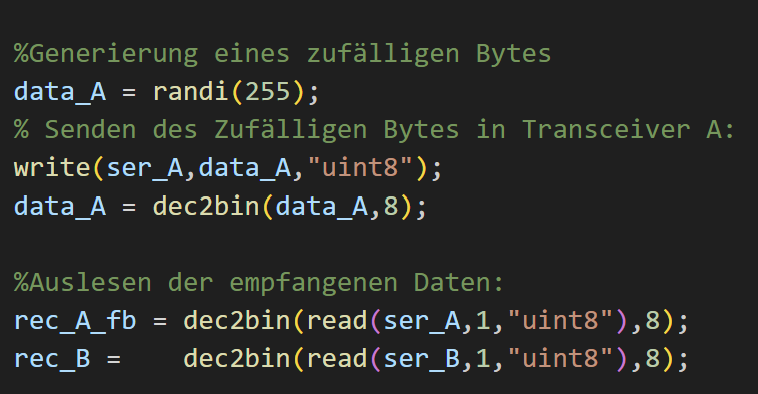
\includegraphics[width=0.5\textwidth]{Pictures/einlesenMatlab.png}
    \caption{Senden/Empfangen}
    \label{fig:matlab_example}
\end{figure}
In diesem Code wird zuerst eine random zahl erzeugt die bis 255 geht.
Um diese in Binärer form daszustellen werden 8Bit benötigt.
\\
Nachdem die Daten gesendet wurden, werden sie vom empfänger und auch Sender eingelesen.
Danach werden sie in die Variable rec\_A\_fb für den Sender selbst und rec\_B für den Empfänger gespeichert.
\\
Nun wird genauer betrachtet wie die Bitfehlerrate berrechnet wird:
\begin{figure}[H]
    \centering
    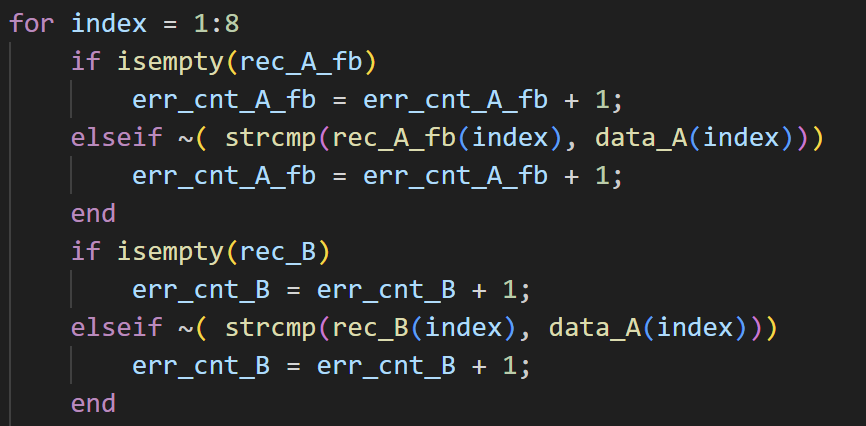
\includegraphics[width=0.5\textwidth]{Pictures/vergleich.png}
    \caption{Bitfehlerrate berrechnung}
    \label{fig:bitfehler}
\end{figure}
Wir iterrieren über jedes Bit also insgesamt acht mal.
Die fehler anzahl werden in err\_cnt\_A\_fb und err\_cnt\_B gespeichert.
Konnten gar keine Daten empfangen werden wird jeweilger Counter auf 8 hochgezählt.
Der intressantere Part ist das vergleichen der gesendeten und empfangenen Daten.
Stimmen diese nicht überein wird ebenfalls der error Counter hochgezählt.
Zum Schluss wird der BER berrechnet und ausgegeben.
Um die genauigkeit zu erhöhen wird das mehrfach wiederholt ebenso wird auch der Sender und Empfänger vertauscht.
Das wurde hier der Übersichtshabler und symmetrie nicht genauer betrachtet.




\section{Pegelplanrechnung}
Die Idee: Wir wollen schauen wann der abstand noch Reicht um die Daten zu empfangen.
Das heißt am ender der empfänger Kette muss ein stark genuges Signal ankommen, damit der Komperator schalten kann.
Damit könnnen wir von hinten nach vorne Rechnen, und herausfinden welche Leistung am empfänge anliegen muss,
damit der Komperator schalten kann.

Aus Versuch fünf ist die Komperator Schwellspannung die bei etwa $V_{Schwell} = 0,822~V$ liegt bekannt.

Als nächstes können wir mithilfe der Analogverstärker kennlinie bzw. der Übertragungsfunktion die Spannung am Kondensator C22 berechnen.
Wenn wir ein Ausgangssignal von $V_{out} = 0,822~V$ annehmen, können wir die Eingangsspannung $V_{in}$ berechnen.

\begin{figure}
    \centering
    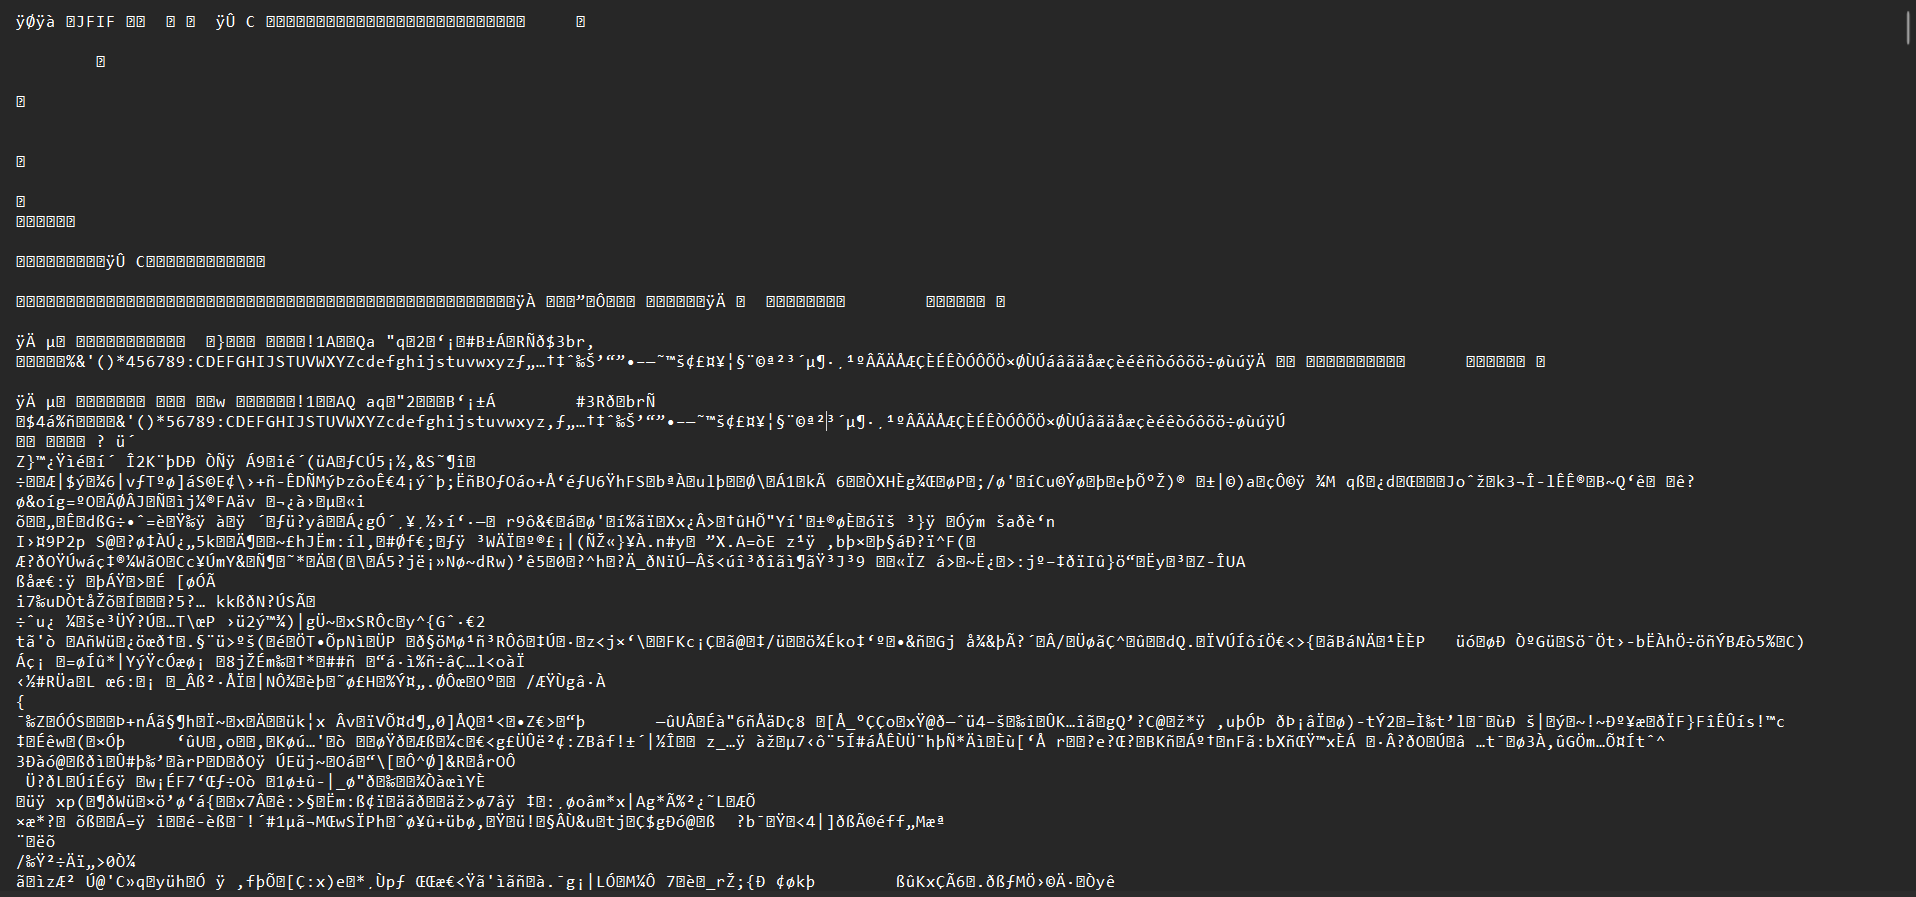
\includegraphics[width=0.8\textwidth]{Pictures/memeASCII.png}
    \caption{Analogverstärker Kennlinie}
    \label{fig:AnalogverstärkerKennlinie}
\end{figure}
Die Formel der Sensititvität des Analogverstärker lautet:
\begin{equation}
    V_\text{out} = k \cdot \sqrt{P_\text{in}} - V_\text{offset}
\end{equation}
Umgestellt nach $P_\text{in}$ ergibt sich:
\begin{equation}
    P_\text{in} = \left(\frac{V_\text{out} + V_\text{offset}}{k}\right)^2
\end{equation}
Mit den Empirisch bestimmten Werten:
\begin{equation}
    P_\text{in} = \left(\frac{xxxxxxxxxxxxxxxxxxxxxxx~V + 368,27~mV}{9,72~\frac{V}{\sqrt{mW}}}\right)^2
\end{equation}
Somit wissen wir nun Welche Leistung am Eingang des Empfängers anliegen muss, damit ein gesendet Signal auch empfangen werden kann.
\begin{equation}
    P_{TX} = P_{RX} + G_{Antenne} + G_{Antenne}
\end{equation}
\subsection{Rekapitulation des Link-Budgets}
\subsection{Rekapitulation der Sensitivität}
\subsection{Berechnung des Pegelplans}